\documentclass[runningheads]{llncs}
%
\usepackage[T1]{fontenc}
\usepackage{graphicx}


\begin{document}
%
\title{Contribution Title}
%
%\titlerunning{Abbreviated paper title}
% If the paper title is too long for the running head, you can set
% an abbreviated paper title here
%
\author{First Author\inst{1}\orcidID{0000-1111-2222-3333} \and
Second Author\inst{2,3}\orcidID{1111-2222-3333-4444} \and
Third Author\inst{3}\orcidID{2222--3333-4444-5555}}
%
\authorrunning{F. Author et al.}
% First names are abbreviated in the running head.
% If there are more than two authors, 'et al.' is used.
%
\institute{Princeton University, Princeton NJ 08544, USA \and
Springer Heidelberg, Tiergartenstr. 17, 69121 Heidelberg, Germany
\email{lncs@springer.com}\\
\url{http://www.springer.com/gp/computer-science/lncs} \and
ABC Institute, Rupert-Karls-University Heidelberg, Heidelberg, Germany\\
\email{\{abc,lncs\}@uni-heidelberg.de}}
%
\maketitle
%
\begin{abstract}
	...

\keywords{First keyword  \and Second keyword \and Another keyword.}
\end{abstract}


\section{Introduction}
\label{sec:introduction}



% ############################# %
% Espace réservé aux encadrants %
% ############################# %



\section{Modèle informel}
\label{sec:informal-model}



\section{Modèle formel}
\label{sec:formal-model}

\section{Formalisation en TLA}
\label{sec:tla-formalisation}

\section{Composition}
\label{sec:composition}

\section{Expériences}
\label{sec:experiments}

\section{Conclusion}
\label{sec:conclusion}

%temporaire, histoire d'avoir le sommaire en tête
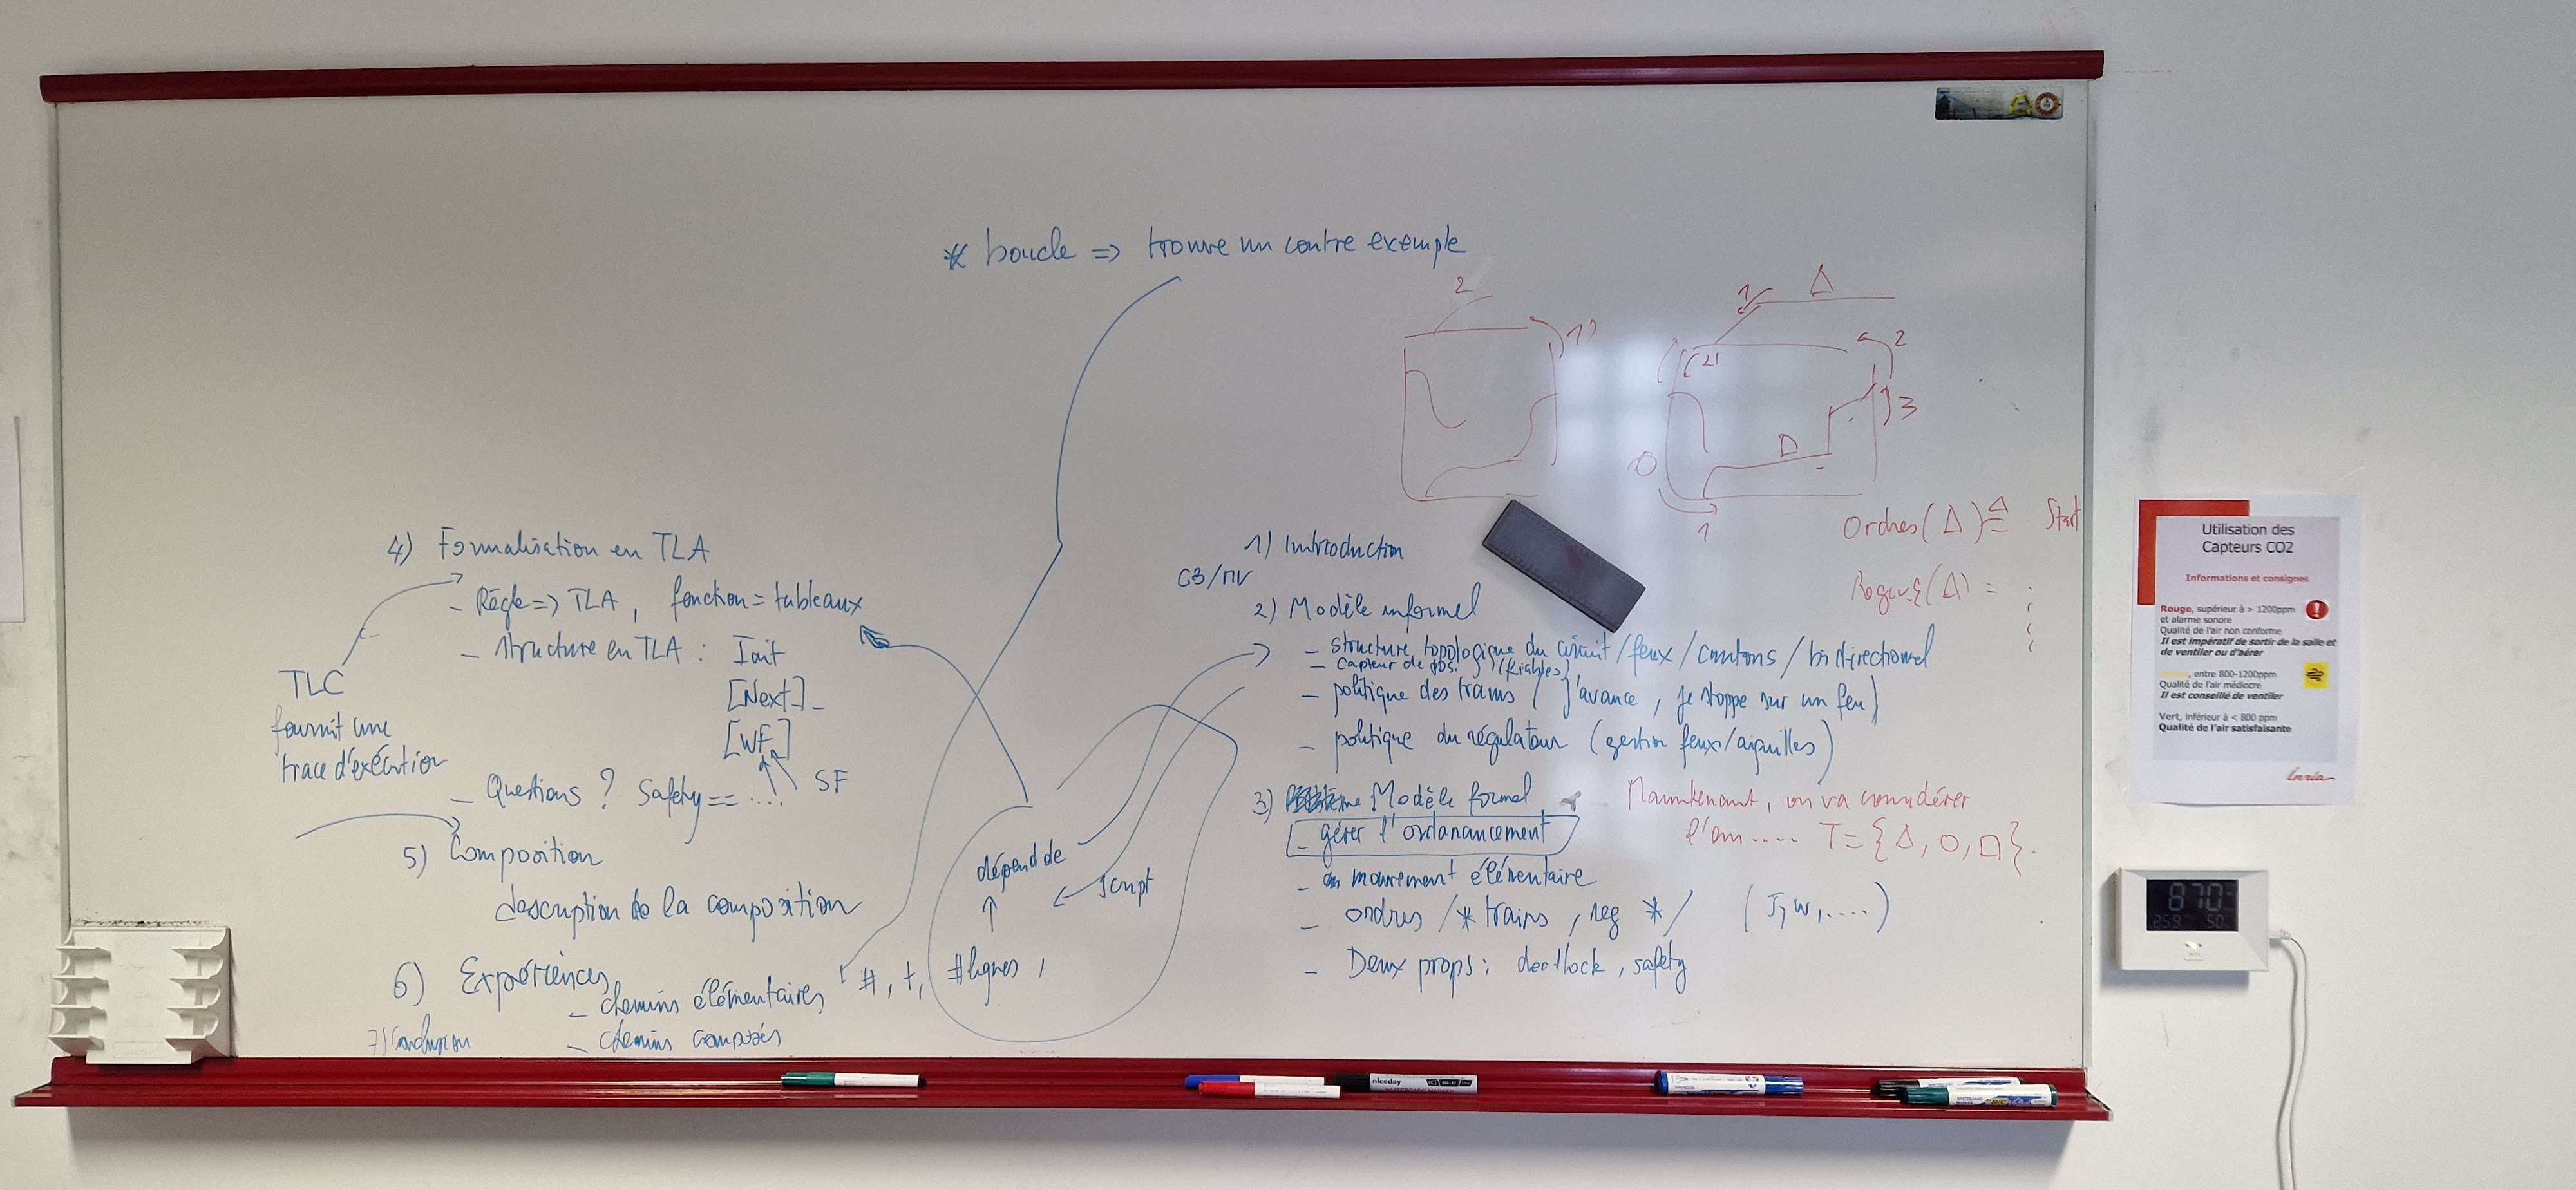
\includegraphics[scale=0.1]{img/sommaire_tableau.jpg}


\bibliographystyle{splncs04}
\bibliography{refs}
\end{document}
